\documentclass{standalone}
\usepackage{tikz}
\usepackage{ctex,siunitx}
\usepackage{tkz-euclide}
\usepackage{amsmath}
\usetikzlibrary{patterns, calc}
\usetikzlibrary {decorations.pathmorphing, decorations.pathreplacing, decorations.shapes,}
\begin{document}
\small
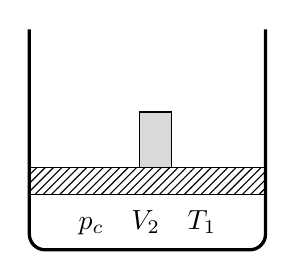
\begin{tikzpicture}[>=stealth,xscale=2,yscale=0.7]
  \draw [rounded corners=0.2cm, very thick](-.5,2)--(-.5,-2)--(1,-2)--(1,2);
  \draw [pattern=north east lines](-.5,-1) rectangle (1,-0.5);	
  \node at (.5/2, -1.5){$p_c\quad V_2\quad T_1$};
  \draw [fill=gray!30](0.2,-.5) rectangle(0.4,.5);
  % \draw[->](1.1,0)--node [above]{等容}(1.9,0);
\end{tikzpicture}
\end{document}